\subsection{Product Details Page}
\bigskip
\paragraph{}
In Product Details page, there is a table that contains all the products' detailed information like product ID, description, categories, qty, etc. Website admins can see and modify the products information, add new product or delete an existing one. Select one product from the table and then click Edit button, admins can edit that product's information. Or by clicking the Delete button, admin can delete one existing product from website and also from the database. On the other hand, if admin want to add new product to the system, he/she click the Add button and add product.
\bigskip
\bigskip
\bigskip
\begin{figure}[h]
\centerline{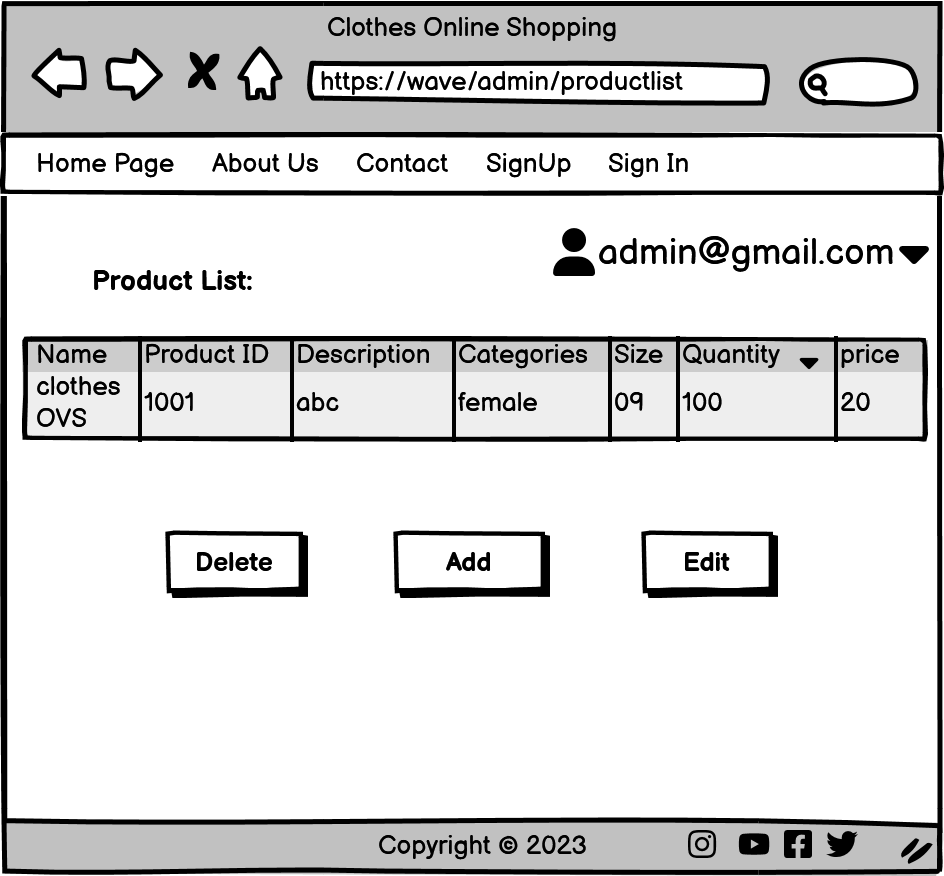
\includegraphics[scale=1.]{images/Product Details.png}}
\caption{Product Details Page}
\label{fig}
\end{figure}

\newpage
\subsection{Add Product Page}
\bigskip
\paragraph{}
In Add Product page, admin will fill manually the required fields; product ID, product name, price, quantity, size, description, etc and also image(s) of that product. Then, click the Add button at the end of the page. By clicking the Add button, new product is created and added to the system and database. Customers can add this new product to their cart. 

\bigskip
\bigskip
\bigskip
\begin{figure}[h]
\centerline{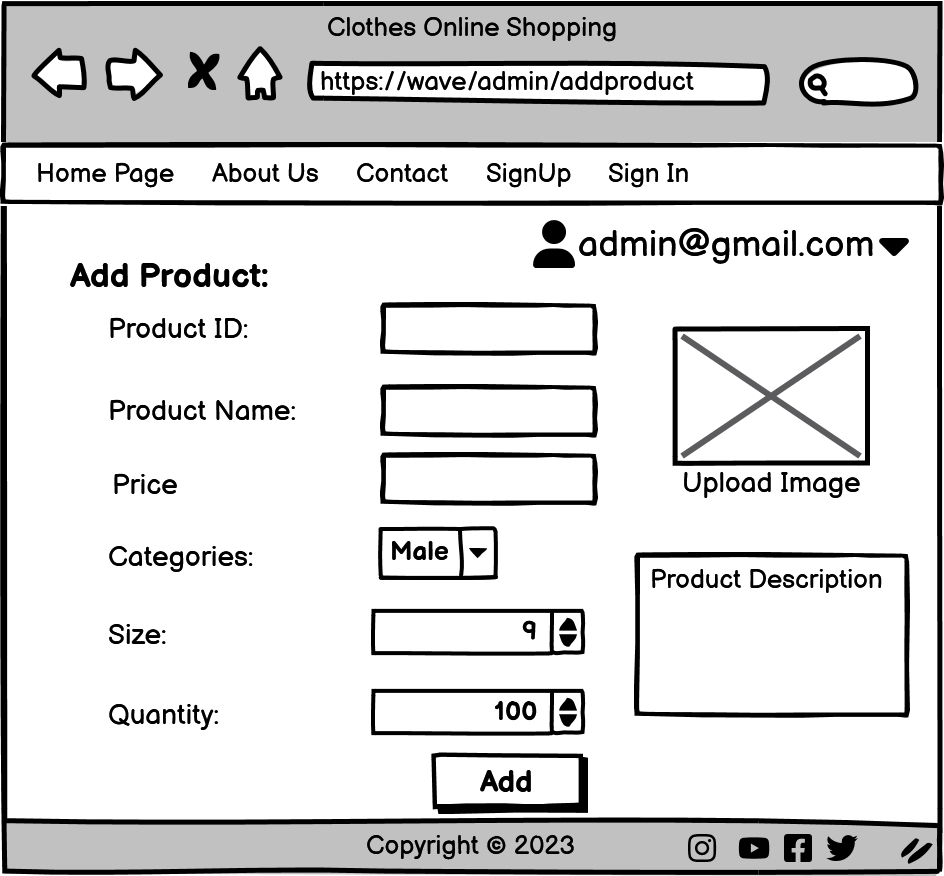
\includegraphics[scale=1.]{images/Add Product.png}}
\caption{Add Product Page}
\label{fig}
\end{figure}

\newpage
\subsection{Edit Product Page}
\bigskip
\paragraph{}
In Edit Product page, admins can see a product's information in details and change them. After changing the fields, they click the Edit button and submit the changes to the database. 
\bigskip
\bigskip
\bigskip
\begin{figure}[h]
\centerline{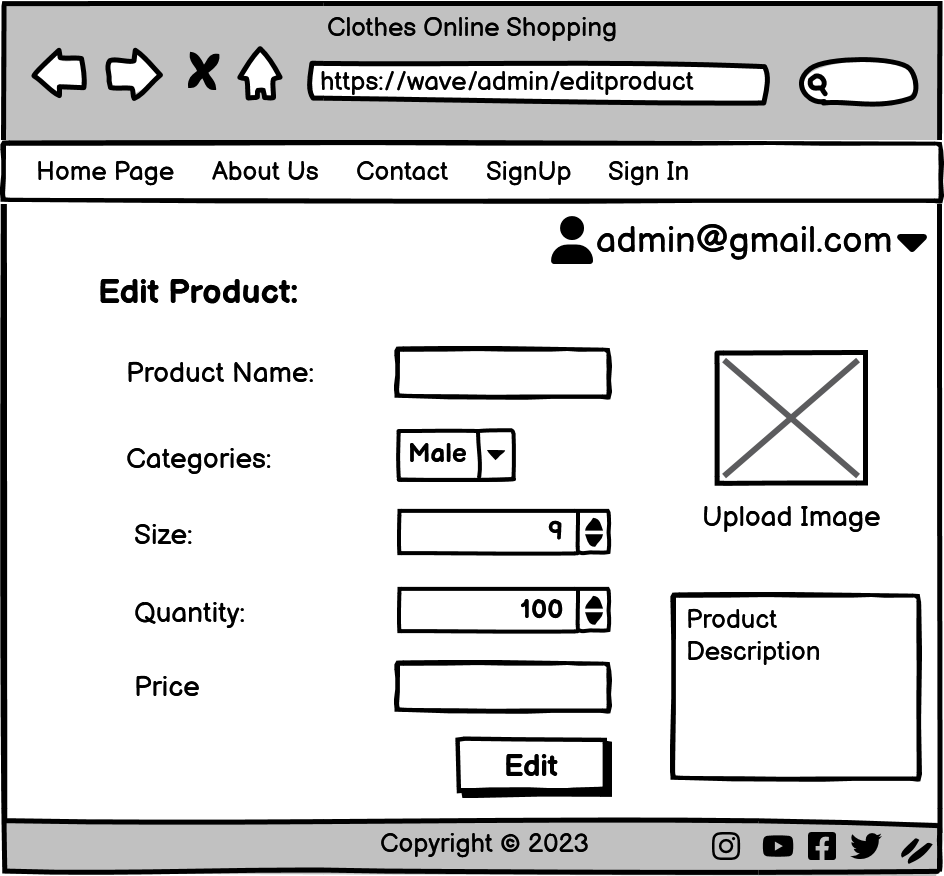
\includegraphics[scale=1.]{images/Edit Product.png}}
\caption{Edit Product Page}
\label{fig}
\end{figure}